\documentclass[border=3pt]{standalone}
% Preâmbulo compartilhado pelos diagramas TikZ da aula 14 (SLAM com EIF)
\usepackage[T1]{fontenc}
\usepackage[utf8]{inputenc}
\usepackage{lmodern}
\usepackage{amsmath}
\usepackage{xcolor}
\usepackage{tikz}
\usetikzlibrary{arrows.meta,angles,quotes,decorations.pathmorphing,decorations.pathreplacing,calc,
                positioning,shapes.geometric,shapes.misc,backgrounds,fit,
                math}

% Paleta (mesma dos SVGs originais)
\definecolor{dblue}{HTML}{2A5B8C}
\definecolor{dorange}{HTML}{B3541E}
\definecolor{dgreen}{HTML}{4A7C59}
\definecolor{dred}{HTML}{9C4B4B}
\definecolor{dcream}{HTML}{F4F1EA}
\definecolor{dshade}{HTML}{DDD7C9}

% Função gaussiana (não normalizada por padrão de escala visual)
\pgfmathdeclarefunction{gauss}{3}{%
  \pgfmathparse{1/(#3*sqrt(2*pi))*exp(-((#1-#2)^2)/(2*#3^2))}%
}

% Estilos comuns (prefixo d... para não colidir com chaves internas do pgf)
\tikzset{
  >={Stealth[length=2mm]},
  dguide/.style={gray!55, dashed, line width=0.4pt},
  daxis/.style={gray!60, line width=0.7pt, ->},
  dbody/.style={fill=black!3, draw=black!80, line width=1pt},
  dacc/.style={draw=dblue, line width=1pt},
  dlbl/.style={black!55, font=\small},
  dsub/.style={black!45, font=\footnotesize},
  dstate/.style={circle, draw=black!80, fill=dcream, line width=1pt,
                 minimum size=17mm, font=\large, inner sep=1pt},
  dobs/.style={circle, draw=black!80, fill=dshade, line width=1pt,
               minimum size=14mm, font=\large, inner sep=1pt},
  dbox/.style={rounded corners=2pt, draw=black!80, fill=dcream, line width=1pt,
               align=center, inner sep=6pt},
  dop/.style={circle, draw=black!80, fill=white, line width=1pt,
              minimum size=6mm, inner sep=0pt, font=\small},
  dtrans/.style={->, dblue, line width=1pt},
  dmeas/.style={->, dorange, line width=1pt},
  dcurve/.style={line width=1pt, dblue},
  dcurveb/.style={line width=1.4pt, dorange},
}

\begin{document}
\hyphenpenalty=10000 \exhyphenpenalty=10000 \tolerance=9999 \emergencystretch=3em
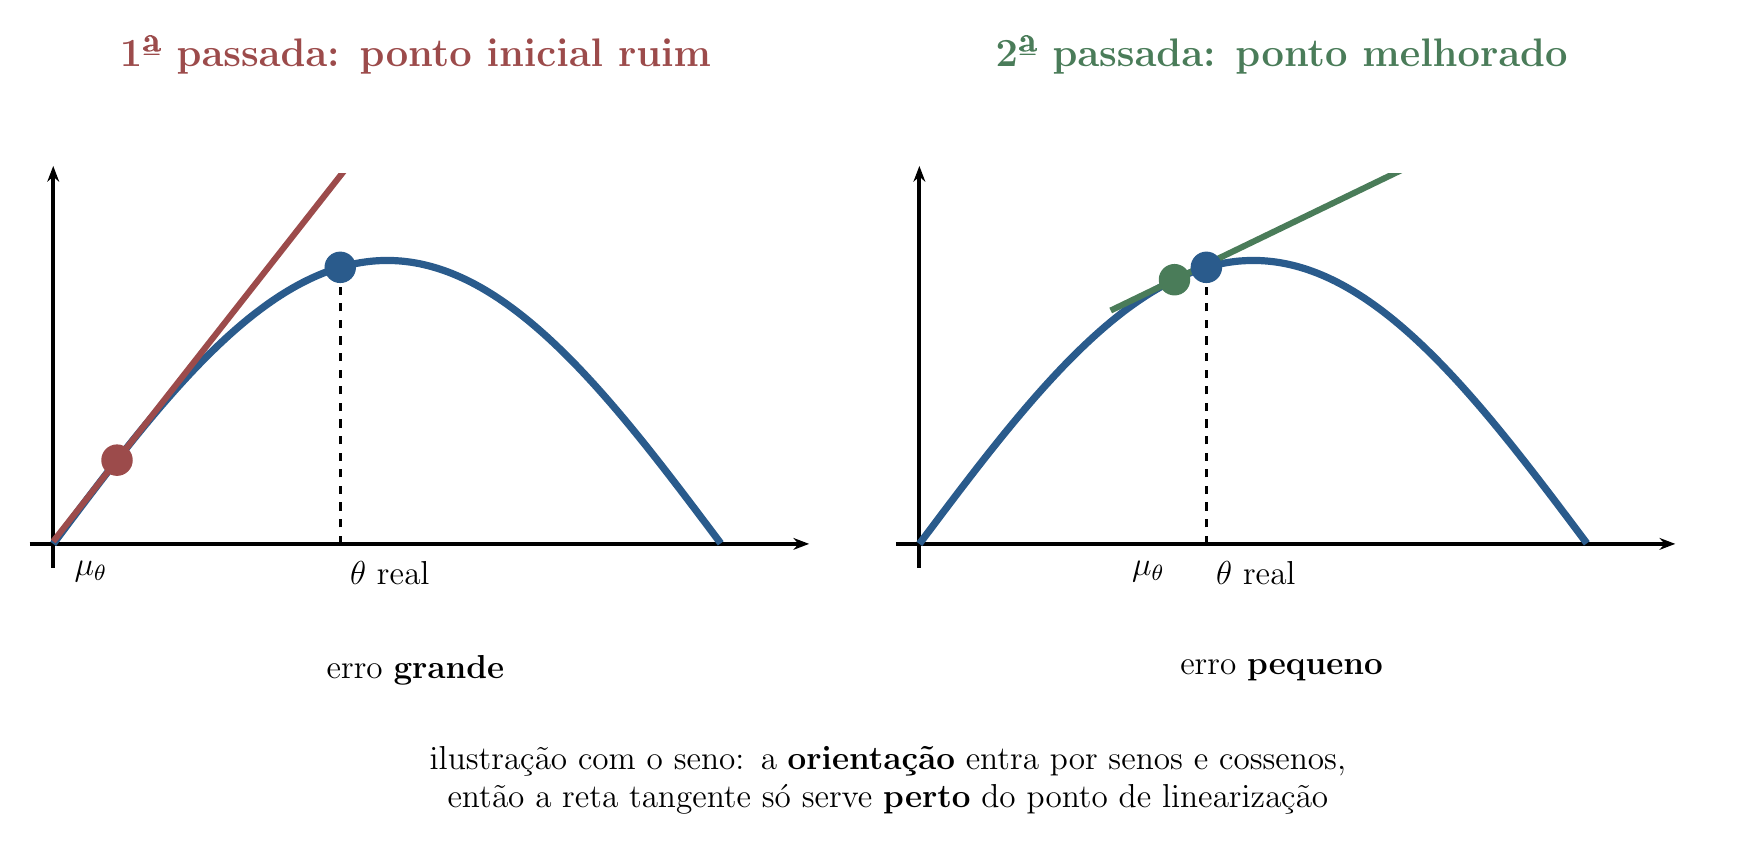
\begin{tikzpicture}[x=1cm,y=1cm]
\def\tc{1.35}
\foreach \o/\a/\col/\tit/\res/\am/\bm in {0/0.3/dred/{1ª passada: ponto inicial ruim}/{erro \textbf{grande}}/north east/north west, 11.0/1.2/dgreen/{2ª passada: ponto melhorado}/{erro \textbf{pequeno}}/north east/north west} {
  \node[font=\Large\bfseries, text=\col] at ({\o+4.6},6.2) {\tit};
  \draw[line width=1.4pt, ->] ({\o-0.3},0) -- ({\o+9.6},0); \draw[line width=1.4pt, ->] ({\o},-0.3) -- ({\o},4.8);
  \draw[domain=0:3.14, samples=70, smooth, line width=2.6pt, draw=dblue] plot ({\o+\x*2.7},{3.6*sin(\x r)});
  \begin{scope}\clip ({\o-0.2},-0.2) rectangle ({\o+9.6},4.7);
  \draw[domain=\a-0.3:\a+1.8, samples=2, line width=2.2pt, draw=\col] plot ({\o+\x*2.7},{3.6*(sin(\a r)+cos(\a r)*(\x-\a))});
  \end{scope}
  \fill[\col] ({\o+\a*2.7},{3.6*sin(\a r)}) circle (0.2);
  \draw[dashed, line width=1.2pt] ({\o+\tc*2.7},0) -- ({\o+\tc*2.7},{3.6*sin(\tc r)});
  \fill[dblue] ({\o+\tc*2.7},{3.6*sin(\tc r)}) circle (0.2);
  \node[font=\large, anchor=\bm] at ({\o+\tc*2.7},-0.1) {$\theta$ real};
  \node[font=\large, anchor=\am] at ({\o+\a*2.7},-0.1) {$\mu_\theta$};
  \node[font=\large, text width=9cm, align=center] at ({\o+4.6},-1.6) {\res};}
\node[font=\large, text width=21cm, align=center] at (10.6,-3.0) {ilustração com o seno: a \textbf{orientação} entra por senos e cossenos, então a reta tangente só serve \textbf{perto} do ponto de linearização};
\end{tikzpicture}
\end{document}
